\documentclass[11pt]{exam}
\printanswers
% \documentclass[a4paper,10pt]{article}
\usepackage{tikz}
\usetikzlibrary{arrows,positioning,shapes.geometric}
\usepackage{amsmath,amssymb,complexity}
\usepackage{datetime,enumerate,palatino}
\usepackage{setspace}

\usepackage[utf8]{inputenc}
\usepackage[numbers]{natbib}
\usepackage{mathpartir}
\usepackage{mathtools}
\usepackage{mathpartir}
\usepackage{stmaryrd}
\usepackage{amsfonts}
\usepackage{amsmath}
\usepackage{amsthm}
\usepackage{listings}
\usepackage{multirow}
\usepackage[T1]{fontenc}
\usepackage{helvet}
\usepackage{array}
\usepackage{ragged2e}
\usepackage{tfrupee}  

\textwidth6in

\setlength{\topmargin}{0in} \addtolength{\topmargin}{-\headheight}
\addtolength{\topmargin}{-\headsep}

\setlength{\oddsidemargin}{0in}

\oddsidemargin  0.2in \evensidemargin 0.0in %\parindent0em


\newtheorem{theorem}{Theorem}
\newtheorem{lemma}{Lemma}
\newtheorem{corollary}{Corollary}
\newcommand\tab[1][1cm]{\hspace*{#1}}

%opening
\title{Your Name\\ Your ID}
\author{}
\date{}
\begin{document}

\hrule
\vspace{3mm}
\noindent
{\sf CS6370 : Natural Language Processing  \hfill Assignment \#2 }
\vspace{3mm}
\noindent
% {\sf Topic: OFWs and PRGs\hfill Due on : $29^{th}$ Dec, 2020}
% \vspace{3mm}
\hrule

% uncomment the lines below and fill name and roll number of teammates here

\hrule
\vspace{3mm}
\noindent
{\sf Roll No: CS14B017\hfill Full Name: Manohar Mulle} 
\vspace{3mm}\\
\noindent
{\sf Roll No: CS14B043\hfill Full Name: Harshal Gawai} 
\vspace{3mm}
\hrule

\begin{questions}
\question Now that the Cranfield documents are pre-processed, our search engine needs a data
structure to facilitate the ’matching’ process of a query to its relevant documents. Let’s
work out a simple example. Consider the following table of term frequencies for three
documents. Give an inverted index representation for the same.
    \begin{center}
    \begin{tabular}{ |c||c|c|c| } 
     \hline
     &\textbf{Doc 1} & \textbf{Doc 2} & \textbf{Doc 3} \\ 
     \hline\hline
     \textbf{cat}& 4 & 2 & 1 \\ 
     \hline
     \textbf{dog}& 3 & 0 & 3 \\ 
     \hline
     \textbf{animal}& 1 & 3 & 3 \\ 
     \hline
    \end{tabular}
    \end{center}
    
\begin{solution}
    Given term frequency matrix:\\
    $\implies$
    \begin{center}
    \begin{tabular}{ |c||c|c|c| } 
     \hline
     &\textbf{Doc 1} & \textbf{Doc 2} & \textbf{Doc 3} \\ 
     \hline\hline
     \textbf{cat}& 4 & 2 & 1 \\ 
     \hline
     \textbf{dog}& 3 & 0 & 3 \\ 
     \hline
     \textbf{animal}& 1 & 3 & 3 \\ 
     \hline
    \end{tabular}
    \end{center}
    Sort terms alphabetically\\
    $\implies$
    \begin{center}
    \begin{tabular}{ |c||c|c|c| } 
     \hline
     &\textbf{Doc 1} & \textbf{Doc 2} & \textbf{Doc 3} \\ 
     \hline\hline
     \textbf{animal}& 1 & 3 & 3 \\ 
     \hline
     \textbf{cat}& 4 & 2 & 1 \\ 
     \hline
     \textbf{dog}& 3 & 0 & 3 \\ 
     \hline
    \end{tabular}
    \end{center}
    Now, Sort documents (will remain same)\\
    $\implies$
    \begin{center}
    \begin{tabular}{ |c||c|c|c|} 
     \hline
     &\textbf{Doc 1} & \textbf{Doc 2} & \textbf{Doc 3} \\ 
     \hline\hline
     \textbf{animal}& 1 & 3 & 3 \\ 
     \hline
     \textbf{cat}& 4 & 2 & 1 \\ 
     \hline
     \textbf{dog}& 3 & 0 & 3 \\ 
     \hline
    \end{tabular}
    \end{center}
    
    Getting doc frequencies and posting lists for each term to get inverted index represents\\
    $\implies$\\

    \begin{center}
    \begin{tabular}{ c|c c c } 
     \hline
     \textbf{Term} & \textbf{Doc. freq.} & \textbf{} & \textbf{Posting list} \\
     \hline\\
     \textbf{animal}& 3 & $\rightarrow$ & 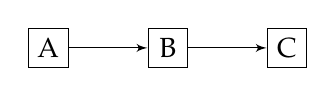
\begin{tikzpicture}[>=latex']
        \tikzset{block/.style= {draw, rectangle, align=center,minimum width=0.5cm,minimum height=0.5cm},
        rblock/.style={draw, shape=rectangle,rounded corners=1.5em,align=center,minimum width=2cm,minimum height=1cm},
        input/.style={ % requires library shapes.geometric
        draw,
        trapezium,
        trapezium left angle=60,
        trapezium right angle=120,
        minimum width=1cm,
        align=center,
        minimum height=1cm
    },
        }
        \node [block]  (start) {A};
        \node [block, right =1cm of start] (acquire) {B};
        \node [block, right =1cm of acquire] (rgb2gray) {C};
%% paths
        \path[draw,->] (start) edge (acquire)
                    (acquire) edge (rgb2gray)
                    ;
    \end{tikzpicture} \\ 
     
     \textbf{cat}& 3 & $\rightarrow$ & 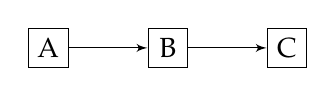
\begin{tikzpicture}[>=latex']
        \tikzset{block/.style= {draw, rectangle, align=center,minimum width=0.5cm,minimum height=0.5cm},
        rblock/.style={draw, shape=rectangle,rounded corners=1.5em,align=center,minimum width=2cm,minimum height=1cm},
        input/.style={ % requires library shapes.geometric
        draw,
        trapezium,
        trapezium left angle=60,
        trapezium right angle=120,
        minimum width=1cm,
        align=center,
        minimum height=1cm
    },
        }
        \node [block]  (start) {A};
        \node [block, right =1cm of start] (acquire) {B};
        \node [block, right =1cm of acquire] (rgb2gray) {C};
%% paths
        \path[draw,->] (start) edge (acquire)
                    (acquire) edge (rgb2gray)
                    ;
    \end{tikzpicture} \\ 
     
     \textbf{dog}& 2 & $\rightarrow$ & 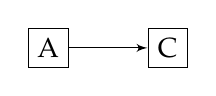
\begin{tikzpicture}[>=latex']
        \tikzset{block/.style= {draw, rectangle, align=center,minimum width=0.5cm,minimum height=0.5cm},
        rblock/.style={draw, shape=rectangle,rounded corners=1.5em,align=center,minimum width=2cm,minimum height=1cm},
        input/.style={ % requires library shapes.geometric
        draw,
        trapezium,
        trapezium left angle=60,
        trapezium right angle=120,
        minimum width=1cm,
        align=center,
        minimum height=1cm
    },
        }
        \node [block]  (start) {A};
        \node [block, right =1cm of start] (acquire) {C};
%% paths
        \path[draw,->] (start) edge (acquire)
                    ;
    \end{tikzpicture} \\ \\
     \hline
    \end{tabular}
    \end{center}
\end{solution}
%%%%%%%%%%%%%%%%%%%            222222222222222       %%%%%%%%%%%%%%%%%%%%%%%%%%%%%%%%%%%%%%%%%%%%%%%%%%%%%%%%%%%%%%%
\question Next, we must proceed on to finding a representation for the text documents. In the class,
we saw about the TF-IDF measure. What would be the TF-IDF vector representations for
the documents in the above table? State the formula used.
\begin{solution}
    Given term frequency matrix:\\
    $\implies$
    \begin{center}
    \begin{tabular}{ |c||c|c|c| } 
     \hline
     &\textbf{Doc 1} & \textbf{Doc 2} & \textbf{Doc 3} \\ 
     \hline\hline
     \textbf{cat}& 4 & 2 & 1 \\ 
     \hline
     \textbf{dog}& 3 & 0 & 3 \\ 
     \hline
     \textbf{animal}& 1 & 3 & 3 \\ 
     \hline
    \end{tabular}
    \end{center}
    Let TF-IDF vector representations for the documents in the above table be\\
    \begin{align}
        \overline{D}_j = \sum_{t\in \mathbb{T}}w_{t,d}\hat{T_t}
    \end{align}
    Where $d\in \mathbb{D} = \{A,B,C\}$\\
    $t\in \mathbb{T} = \{cat, dog, animal\}$\\
    $\hat{T_t}$ = unit vector corresponding to term $t \in \mathbb{T}$ that is orthogonal to $\hat{T_t}$ , $\forall t' \in \mathbb{T} \textbackslash \{j\}$\\
    $w_{t,d}$ = TF-IDF measure weight of (t,d) term-document pair\\\\
    Now, we will find $w_{t,d}$ \tab $\forall d \in \mathbb{D}$ and $\forall t \in \mathbb{T}$\\
    \begin{align*}
        w_{t,d} &= tf{\text -}idf_{t,d}\\
        &= tf_{t,d} * idf_t\\
        idf_t = log{\frac{N}{df_t}}
    \end{align*}
    here, $tf_{t,d} =$ term frequency of term $t$ in document $d$\\
    and $idf_t = $ inverse document frequency of term $t$\\
    $N = $ total no. of documents in which term $t$ appears\\
    $N = |\textbf{D}| = 3$
    
    Count $(t,d)$ is already given:\\
    \begin{center}
    \begin{tabular}{ |c||c|c|c| } 
     \hline
     &\textbf{A} & \textbf{B} & \textbf{C} \\ 
     \hline\hline
     \textbf{cat}& 4 & 2 & 1 \\[1em]
     \hline
     \textbf{dog}& 3 & 0 & 3 \\[1em] 
     \hline
     \textbf{animal}& 1 & 3 & 3 \\[1em] 
     \hline
    \end{tabular}
    \end{center}
    
    Calculating term frequency $tf_{t,d}$ :
    \begin{center}
    \begin{tabular}{ |c||c|c|c|c|c| } 
     \hline
     &\textbf{A} & \textbf{B} & \textbf{C} & \textbf{df} & \textbf{$idf_t = log\dfrac{N}{t_f}$}\\[1em]
     \hline\hline
     \textbf{cat}& $\dfrac{4}{8}$ & $\dfrac{2}{5}$ & $\dfrac{1}{7}$ & $3$ & $log\dfrac{3}{3} = 0$\\[1em]
     \hline
     \textbf{dog}& $\dfrac{3}{8}$ & $\dfrac{0}{5}$ & $\dfrac{3}{7}$ & 2 & $log\dfrac{3}{2}=log1.5 = 0.176$\\[1em]
     \hline
     \textbf{animal}& $\dfrac{1}{8}$ & $\dfrac{3}{5}$ & $\dfrac{3}{7}$ & 3 & $log\dfrac{3}{3} = 0$\\[1em]
     \hline
    \end{tabular}
    \end{center}
    
    Calculating $tf{\text -}idf_{t,d}$ measure:\\
    \begin{center}
        \begin{tabular}{|c||c|c|c|}
        \hline
             &\textbf{A} & \textbf{\tab B\tab} & \textbf{C}  \\
             \hline\hline
             \textbf{cat} & $0$ & $0$ & $0$\\[1em]
             \hline
             \textbf{dog} & $\dfrac{3}{8}*log1.5 = 0.066$ & $0$ & $\dfrac{3}{7}*log1.5 = 0.076$\\[1em]
             \hline
             \textbf{animal} & $0$ & $0$ & $0$\\[1em]
             \hline
        \end{tabular}
    \end{center}
    % The Inverse of above matrix i.e. $(tf{\text -}idf_{t,d})^{-1}$ is:\\
    \begin{center}
        \begin{tabular}{|c||c|c|c|}
        \hline
            \tab &\textbf{cat} & \textbf{dog} & \textbf{animal}  \\
             \hline\hline
             \textbf{A} & $0$ & $\dfrac{3}{8}*log1.5 = 0.066$ & $0$\\[1em]
             \hline
             \textbf{B} & $0$ & $0$ & $0$\\[1em]
             \hline
             \textbf{C} & $0$ & $\dfrac{3}{8}*log1.5 = 0.076$ & $0$\\[1em]
             \hline
        \end{tabular}
    \end{center}
    $\therefore$ the $tf{\text -}idf_{t,d}$ vector representation of the documents is\\
    \begin{align*}
        \overline{D}_A &= 0 \cdot \hat{T}_{cat} + 0.066 \cdot \hat{T}_{dog} + 0 \cdot \hat{T}_{animal}\\
        \overline{D}_B &= 0 \cdot \hat{T}_{cat} + 0 \cdot \hat{T}_{dog} + 0 \cdot \hat{T}_{animal}\\
        \overline{D}_C &= 0 \cdot \hat{T}_{cat} + 0.076 \cdot \hat{T}_{dog} + 0 \cdot \hat{T}_{animal}\\
    \end{align*}
    \end{solution}
%%%%%%%%%%%%%%%%%%%%%%%%%%%%333333333333%%%%%%%%%%%%%%%%%%%%%%%%%%%%%%%%%%%%%%%%%%%%%%%%%%%%%%%%%%%%%%%%%%%%%%%%%%%%%%%%%%%%%%%%%%%%%%%%%%
\question Suppose the query is "dog", which documents would be retrieved based on the inverted
index constructed before?
\begin{solution}
    \begin{center}
    \begin{tabular}{ c|c c c } 
     \hline
     \textbf{Term} & \textbf{Doc. freq.} & \textbf{} & \textbf{Posting list} \\
     \hline\\
     \textbf{animal}& 3 & $\rightarrow$ & 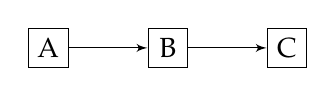
\begin{tikzpicture}[>=latex']
        \tikzset{block/.style= {draw, rectangle, align=center,minimum width=0.5cm,minimum height=0.5cm},
        rblock/.style={draw, shape=rectangle,rounded corners=1.5em,align=center,minimum width=2cm,minimum height=1cm},
        input/.style={ % requires library shapes.geometric
        draw,
        trapezium,
        trapezium left angle=60,
        trapezium right angle=120,
        minimum width=1cm,
        align=center,
        minimum height=1cm
    },
        }
        \node [block]  (start) {A};
        \node [block, right =1cm of start] (acquire) {B};
        \node [block, right =1cm of acquire] (rgb2gray) {C};
%% paths
        \path[draw,->] (start) edge (acquire)
                    (acquire) edge (rgb2gray)
                    ;
    \end{tikzpicture} \\ 
     
     \textbf{cat}& 3 & $\rightarrow$ & 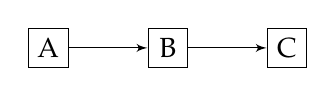
\begin{tikzpicture}[>=latex']
        \tikzset{block/.style= {draw, rectangle, align=center,minimum width=0.5cm,minimum height=0.5cm},
        rblock/.style={draw, shape=rectangle,rounded corners=1.5em,align=center,minimum width=2cm,minimum height=1cm},
        input/.style={ % requires library shapes.geometric
        draw,
        trapezium,
        trapezium left angle=60,
        trapezium right angle=120,
        minimum width=1cm,
        align=center,
        minimum height=1cm
    },
        }
        \node [block]  (start) {A};
        \node [block, right =1cm of start] (acquire) {B};
        \node [block, right =1cm of acquire] (rgb2gray) {C};
%% paths
        \path[draw,->] (start) edge (acquire)
                    (acquire) edge (rgb2gray)
                    ;
    \end{tikzpicture} \\ 
     
     \textbf{dog}& 2 & $\rightarrow$ & 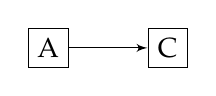
\begin{tikzpicture}[>=latex']
        \tikzset{block/.style= {draw, rectangle, align=center,minimum width=0.5cm,minimum height=0.5cm},
        rblock/.style={draw, shape=rectangle,rounded corners=1.5em,align=center,minimum width=2cm,minimum height=1cm},
        input/.style={ % requires library shapes.geometric
        draw,
        trapezium,
        trapezium left angle=60,
        trapezium right angle=120,
        minimum width=1cm,
        align=center,
        minimum height=1cm
    },
        }
        \node [block]  (start) {A};
        \node [block, right =1cm of start] (acquire) {C};
%% paths
        \path[draw,->] (start) edge (acquire)
                    ;
    \end{tikzpicture} \\ \\
     \hline
    \end{tabular}
    \end{center}
    Based on this inverted index that was constructed in que.1 \textbf{Doc A} and \textbf{Doc C} would be retrieved.
\end{solution}
%%%%%%%%%%%%%%%%%        444444444444444%%%%%%%%%%%%%%%%%%%%%%%%%%%%%%%%%%%%%%%%%%%%%%%%%%%%%%%%%%%%%%%%%%%%%%%%%%%%%%%%%%%%%%%%%%%%%%%
\question Find the cosine similarity between the query and each of the retrieved documents. Rank
them in descending order.
\begin{solution}\\
    The query vector here is\\
    \begin{align*}
        \overline{D}_q &= \sum_{t\in \mathbb{T}}w_{t,d}\hat{T_t}\\
         &= \sum{t\in \mathbb{T}}tf_{t,q}\times idf_t\overline{T}_t
    \end{align*}
    from quesiton 2, for $t="dog$, $idf_t=0.176$

    The given query doc $q$ is a single word doc containing the word "dog"\\
    $\implies$ the term frequency w.r.t. $q$ is $tf_{t,q}=1$ for t="dog"\\
    \tab\tab\tab\tab\tab\tab\tab[4em]$=0$ otherwise\\
    \begin{align}
        \implies \overline{D}_q = 0.176\hat{T}_dog
    \end{align}
    Now, cosine similarity between $\overline{D}_q$ and $\overline{D}_d \forall d \in \mathbb{D}$ is ${\cos \theta}_{(q,d)}$\\
    Now, cosine similarity between $\overline{T}_q$ and $\overline{T}_d$ $\forall \in \{A,B\}$\\
    Cosine similarity between $\overline{T}_q$ and $\overline{T}_d$
    \begin{align*}
        sim(\overline{T}_q, \overline{T}_A) &= \cos \theta_{q,A}\\
        &=\dfrac{\overline{T}_{q}.\overline{T}_A}{|\overline{T}_q| |\overline{T}_A|}\\
        &=1
    \end{align*}
    Cosine similarity between $\overline{T}_q$ and $\overline{T}_B$:\\
    \begin{align*}
        sim(\overline{T}_q,\overline{T}_B) &= \cos\theta_{q,B}\\
        &=\dfrac{\overline{T}_{q}.\overline{T}_B}{|\overline{T}_q| |\overline{T}_B|}\\
        &=1
    \end{align*}
    
\end{solution}
%%%%%%%%%%%%%%      555555555555555555555        %%%%%%%%%%%%%%%%%%%%%%%%%%%
\question Now, you are set to build a real-world retrieval system. Implement an Information Retrieval System for the Cranfield Dataset using the Vector Space Model.
\begin{solution}
    (Implemented in code)
\end{solution}
%%%%%%%%%%%%%       666666666666666666666        %%%%%%%%%%%%%%%%%%%%%%%%%%%
\question (a) What is the IDF of a term that occurs in every document?\\
(b) Is the IDF of a term always finite? If not, how can the formula for IDF be modified to
make it finite?
\begin{solution}\\
    \textbf{Ans. (a)}\\
    IDF i.e. inverse Document frequency of term $t$ is given by:
    \begin{align}
        idf_t = log{\frac{N}{df_t}}
    \end{align}
    here, $df_t$ = document frequency of a term $t$\\
    $N = $ total no. of documents in which term $t$ appears\\
    So, if a term occures in every document $\implies$ $df_t = N$ \\
    
    \begin{align*}
        idf_t &= log{\frac{N}{df_t}}\\
        &= log{\frac{N}{N}}\\
        &=0
    \end{align*}
    $\therefore$ IDF is $0$ if a term occures in every document\\\\
    \textbf{Ans. (b)}\\
    If certain word doesn't appear in any of the documents\\
    $\implies df_t$ (document frequency) is $0$\\\\
    In this case $log\frac{N}{0}$ won't be finite\\
    Hence, IDF of such term will NOT be finite\\\\
    A light modification to above IDF formula so that denominator won't be $0$:
    \begin{align}
        idf_t &= log{\frac{N+1}{df_t+1}}\\
    \end{align}
    Here, $df_t$ for a word that won't appear in any document will be finite.\\
    (\textbf{Note:} $idf_t$ will be high but finite.)
\end{solution}
%%%%%%%%%%%%%%%%        77777777777777777777777777777777777777
\question Can you think of any other similarity/distance measure that can be used to compare vectors
other than cosine similarity. Justify why it is a better or worse choice than cosine similarity
for IR.
\begin{solution}
    %Vector Space Model views documents (and queries) as frequency vectors of words.\\
    One can use the Euclidean distance as a measure that can be used to compare vectors.\\
    Euclidean distance (squared) between $x$,$y$:
    \begin{align}
        (||x-y||)^2=(||x||)^2+(||y||)^2-2<x,y>
    \end{align}
    where,  $x$ and $y$ are two vectors or two documents on the Vector Space\\
    If one don't normalize the vectors to be all the same length then their length will depend on the length of the document. \\
    In document classification we don't want to be biased by the document lengths.\\
    This is one reason why cosine similarity is preferred choice over Euclidean distance. 
\end{solution}
%%%%%%%%%%%%%%%%%       88888888888888888888888888888888888888
\question Why is accuracy not used as a metric to evaluate information retrieval systems?
\begin{solution}
    Accuracy is the simplest model evaluation metric for classification models. It is the percentage of correctly predicted labels.
    \begin{align}
        Accuracy = \frac{Number of correct predictions}{Total number of predictions}
    \end{align}
    We tend to use accuracy because everyone has an idea of what it means rather than because it is the best tool for the task.When using accuracy, we are assign equal cost to false positives and false negatives. \\
    Precision-Recall is a useful measure of success of prediction when the classes are very imbalanced.\\
    In information retrieval, precision is a measure of result relevancy, while recall is a measure of how many truly relevant results are returned.\\
    There are many other metrics for evaluating binary classification systems. Even plotting a graph can be helpful.\\
    There is no single best way to evaluate any system, but different metrics gives different (and valuable) insights into how any classification model performs.
\end{solution}
%%%%%%%%%%%%%%%          999999999999999
\question For what values of $\alpha$ does the $F_{\alpha}$ -measure give more weightage to recall than to precision?
\begin{solution}
    The $F\mbox{-}measure$ is calculated as the harmonic mean of \textbf{precision} and \textbf{recall}, giving each the same weightage. $F\mbox{-}measure$ is given by:
    \begin{align}
        F\mbox{-}measure = \frac{2*precision*recall}{precision+recall}
    \end{align}
    $F_{\alpha}\mbox{-}measure$ is given by:
    \begin{align}
        F_{\alpha}\mbox{-}measure &= \dfrac{1}{\dfrac{\alpha}{precision}+\dfrac{1-\alpha}{recall}}
        %{\text \alpha is given by equation:}
        % where, \alpha &= \frac{1}{1+{\beta}^2}
    \end{align}
    clearly, for $\alpha < 0.5, F_{\alpha}\mbox{-}measure$ gives more weightage to recall than for precision \\
    % $\therefore$ When $\boldsymbol{\alpha < 0.5}$, $F_{\alpha}\mbox{-}measure$ gives more weightage to recall than to precision.
\end{solution}
%%%%%%%%%%%%%%%%        10 10 10 10 10 10 10 10 10 10
\question What is a shortcoming of Precision @ K metric that is addressed by Average Precision @
k?
\begin{solution}
    A limitation of precision@k is that it doesn’t consider the position of the relevant items.\\
    Average Precision is a metric that evaluates whether all of the relevant items selected by the model are ranked higher or not.\\
\end{solution}
%%%%%%%%%%%%%%%         11 11 11 11 11 11 11 11 11 11
\question What is Mean Average Precision (MAP) @ k? How is it different from Average Precision
(AP) @ k ?
\begin{solution}
    \\1. The average precision $AP(q)@K$ for a query $q$ is essentially the precision $@k$ for q with the positions of relevant-retrieved documents taken into account.\\
    2. The same set of retrieved documents gives different $AP(q)@k$ based on different positions of the relevant docs among retrieved documents.\\
    3.The more the relevant docs appear on top of the retrieved list, the higher $AP(q)@k$\\\\
    Mean average precision for a set of queries is the mean of the average precision scores over all queries. \\
    \begin{align}
        MAP = \frac{\sum_{q=1}^{Q}AP(q)}{Q}
    \end{align}
    where,\\
    $Q$ is the total number of queries. \\
    $AP(q)$ is the average precision for query $q$.
\end{solution}
%%%%%%%%%%%%%%%         12 12 12 12 12 12 12 12 12 12
\question For Cranfield dataset, which of the following two evaluation measures is more appropriate
and why? (a) AP (b) nDCG
\begin{solution}
    The DCG accumulated at a particular rank position $p$ is defined as:
    \begin{align}
        DCG_p &= \sum_{i=1}^{p}\frac{rel_i}{log_2(i+1)}\\
        nDCG &= \frac{DCG_p}{IDCG_p}
    \end{align}
    Average Precision assumes binary relevance. Which means an item is either interest or not (i.e. value is 0 or 1). Whereas NDCG allows relevance scores to be any positive real number.\\
    Since Cranfield dataset contains non-binary relevance judgements for queries, nDCG is a better metric than AP as it can make use of more information(relevance values).
\end{solution}
\question (Implemented in Code)
\question (Implemented in Code) %report

%%%%%%%%%%%%%          15 15 15 15 15 15 15 15
\question Analyse the results of your search engine. Are there some queries for which the search
engine’s performance is not as expected? Report your observations.


\question Do you find any shortcoming(s) in using a Vector Space Model for IR? If yes, report them.
\begin{solution}
    Vector Space Model for IR suffers from two major shortcomings:\\
    1. It makes the consideration of all words impractical: since each word is a dimension, considering all words would imply expensive computations in a very high-dimensional space.\\
    2. It assumes that all words are independent.\\
    3. It does not take into consideration neither the semantics nor the context of the of the sentences of the documents.
    
\end{solution}

\question While working with the Cranfield dataset, we ignored the titles of the documents. But,
titles can sometimes be extremely informative in information retrieval, sometimes even
more than the body. State a way to include the title while representing the document as
a vector. What if we want to weigh the contribution of the title three times that of the
document?
\begin{solution}
    Let $\overline{V}_{old}$ be the vector representation of a Doc $d$ just considering terms from its text.\\
    Let $\overline{V}_{d_{title}}$ be the vector representation of title of $d$\\
    Now, one way to include the title while representing $d$ as a vector is, \\
    \begin{align}
        \overline{V}_{d_{new}} = \alpha(\overline{V}_{d_{old}}) + (1-\alpha).\overline{V}_{d_{title}} ,\tab 0\leq\alpha\leq1
    \end{align}
    Giving title 3 times the weight of the document text:
    \begin{align*}
        \implies \tab\tab \frac{1-\alpha}{\alpha} &= 3\\
        \implies \tab\tab\tab \alpha &= 0.25\\
        \implies \tab\tab \overline{V}_{d_{new}} &= 0.25.\overline{V}_{d_{old}} + 0.75.\overline{V}_{d_{title}}
    \end{align*}
    
\end{solution}
\question Suppose we use bigrams instead of unigrams to index the documents, what would be its
advantage(s) and/or disadvantage(s)?
\begin{solution}
    Advantages:\\
    Hits will be more powerful\\
    Helps in retreiving only VERY relevant documents.\\\\
    Disadvantages:\\
    The size of the bigram vocabulary is likely to be very high(worst-case:$O(n^2)$) compared to that of a unigram\\
    There will be less hits. Many times just because 2 words doesn't appear side by side, it doesn't mean that the document is not relevant.\\
\end{solution}

\question In the Cranfield dataset, we have relevance judgements given by the domain experts.
In the absence of such relevance judgements, can you think of a way in which we can
get relevance feedback from the user himself/herself? Ideally, we would like to keep the
feedback process to be non-intrusive to the user. Hence, think of an ’implicit’ way of
recording feedback from the users

\begin{solution}
    One straight-forward way to get relevance feedback is based on the number of clicks a document get as a whole from all the users for a query.\\\\
    This is a non-intrusive way where we don't have to ask users in specific and the entire process(keeping track of user clicks) can be dome in the background.\\\\
    Relevance can be updated(increased/decreased) in a timely manner based on the number of clicks a document gets for a set of "similar" queries in a given period of time
\end{solution}
\end{questions}
\end{document}
